\documentclass{article}

\usepackage[preprint]{neurips_2023}
\usepackage{shortcuts}


\title{Semantic Classification of 3D point clouds with multiscale spherical neighborhoods \\ \vspace{.3cm}
\small{NPM3D project report}
}

\author{%
  Inès ~Vati\thanks{Engineering student from École des Ponts ParisTech, Champs-sur-Marne, France} \\
  MVA, ENS Paris-Saclay, Cachan, France\\
  \texttt{\email{ines.vati@eleves.enpc.fr}}
}

\date{}

\begin{document}
\maketitle

\begin{abstract}
    The project consists in studying the article from Thomas et al. \cite{thomas_semantic_2018} by implementing it and proposing improvements. The goal of the studied article is to classify each point of a 3D point clouds using an innovative approach to design features which will be used to train a random forest classifier. 
    [what i did]
    As no code were provided, the methods were implemented from scratch. The code implemented for this project is available on \url{https://github.com/InesVATI/npm3d-project}. 
\end{abstract}
\textbf{Keywords.} 3D point clouds, semantic classification, multiscale, spherical neighborhoods, Random Forest Classifier


% \section{Introduction}

\section{Proposed method}

In their study \cite{thomas_semantic_2018}, the authors employ a multiscale approach to design informative features, drawing upon the findings of Hackel et al. in 2016 \cite{hackel_fast_nodate}, which demonstrated the improved efficiency of such an approach over adating the scale for each point \cite{weinmann_semantic_2015}. Indeed, using a fixed scale across the scene is inadequate because most scenes contain objects of various sizes. To compute these features, the authors adopt a spherical definition of neighborhoods, incorporating neighbors within a radius that exponentially increases with the scale $s$, denoted as $r_s = r_0 * \phi^s$. This formulation ensures that the neighborhoods appropriately reflect the density of the point cloud. 

Let's consider a set of $N$ points of interest for which we aim to compute the multiscale features. For each scale, the same set of $N_{feats}$ features is computed, as detailed in Table \ref{tab:thomas_feat}. $S$ is the number of scales. The feature computation proceeds through the following steps:

\begin{enumerate}
    \item At scale 0, the eigenvalues and eigenvectors of the covariance matrix of the neighborhood, obtained with an initial radius $r_0$, are computed. Subsequently, the features for each point of interest are derived using the formulas outlined in Table \ref{tab:thomas_feat}.
    \item  For each scale $s$, a grid subsampling is applied to the original cloud using a voxel size of $r/\rho$. Each original point is then assigned to the closest voxel center, inheriting the features of the voxel center for that particular scale. 
    \item The $N_{feats}$ features are computed for each voxel center associated with at least one point of interest, within a spherical neighborhood of radius $r_s = r_0 * \phi^s$.
    \item Consequently, we obtain a feature matrix of size $N \times N_{feats} * S$.
\end{enumerate}
Here, $\phi$ is the ratio between the radius of consecutive neighborhoods and $\rho$ is the ratio between the radius of the spherical neighborhood and the voxel size of the grid subsampling. $\rho$ enables to control the (maximum) number of subsampled points that a neighborhood can contain.

\begin{table}[H]
    \centering
    \begin{tabular}{|c||c|}
    \hline
    \textbf{Feature} & \textbf{Formula} \\
    \hline   
    Sum of eigenvalues & $\sum \lambda_i$ \\[1ex]
    % \hline
    Omnivariance & $(\prod \lambda_i)^{(1/3)}$\\[1ex]
    % \hline
    Eigenentropy & $-\sum \lambda_i \ln(\lambda_i)$\\[1ex]
    % \hline
    Linearity & $\frac{\lambda_1 - \lambda_2}{\lambda_1}$\\[1ex]
    % \hline
    Planarity & $\frac{\lambda_2 - \lambda_3}{\lambda_1}$\\[1ex]
    % \hline
    Sphericity & $\frac{\lambda_3}{\lambda_1}$\\[1ex]
    % \hline
    Change of curvature & $\lambda_1 - \lambda_3$\\[1ex]
    % \hline
    Verticality ($\times2$) & $|\arcsin(\dotp{e_i}{e_z})|_{i=1, 3}$ \\[1ex]
    % \hline
    Absolute moment ($\times6$) & $\frac{1}{|\mathcal{N}|}|\sum_{j\in\mathcal{N}} \dotp{p_j - \mathbf{p}}{e_i}^k|_{k = 1, 2;\; i = 1, 2, 3}$\\[1ex]
    % \hline  
    Vertical moment ($\times2$) & $\frac{1}{|\mathcal{N}|}|\sum_{j\in\mathcal{N}} \dotp{p_j - \mathbf{p}}{e_z}^k|_{k=1, 2}$ \\[1ex]
    % \hline
    Number of points & $|\mathcal{N}|$\\[1ex]
    \hline
    \end{tabular}
    \caption{Geometric features \cite{thomas_semantic_2018} of point $\mathbf{p}$. Here, $N_{feats}=18$ and $\lambda_i$ are the eigenvalues of the covariance matrix of the neighborhood $\mathcal{N}$ of $\mathbf{p}$, sorted in decreasing order. $e_i$ are the corresponding eigenvectors.}
    \label{tab:thomas_feat}
\end{table}

\begin{table}[H]
    \centering
    \begin{tabular}{|c||c|}
        \hline
    \textbf{Feature} & \textbf{Formula} \\
        \hline
        Vertical range & $z_{max} - z_{min} $\\[1ex]
        % \hline
        Height below & $\mathbf{p}_z - z_{min} $ \\[1ex]
        % \hline
        Height above & $z_{max} - \mathbf{p}_z$\\[1ex]
        \hline
    \end{tabular}

    \caption{Additional height features from \cite{hackel_fast_nodate, mohamed_improvement_2022}, where $z_{max} = \umax{j\in\mathcal{N}}p_{j,z}$ and $z_{min} = \umin{j\in\mathcal{N}} p_{j,z}$. $\N$ is the neighborhood of point $\mathbf{p}$.}
    \label{tab:height_feat}
\end{table}

\section{Experiments and results}
I used two datasets to test the method: the Paris-rue-Cassette dataset\footnote{\url{http://data.ign.fr/benchmarks/UrbanAnalysis/}}, a point cloud of 12 million point and the NPM3D dataset\footnote{\url{https://npm3d.fr/benchmark-for-master-course-on-3d-point-clouds}}, that groups three small point cloud whose the MiniLille and MiniParis point clouds. The MiniLille dataset has 1,901,853 and 2,500,428 points and the MiniParis dataset has 4,159,318 points. The NPM3D dataset is used to evaluate how the method generalizes to unseen data. [REF TO THE SECTION]


\subsection{Paris-rue-cassette dataset}
The raw ground truth contained a large number of classes. I had to parse an XML file to group together some label classes to fairly compare the results with those obtained in the articles \cite{thomas_semantic_2018,hackel_fast_nodate,weinmann_semantic_2015}. 

For sake of computation time, I subsampled the point cloud by grid subsampling with a voxel size of 0.1m. The resulting point cloud has 1,288,215 points. The label of each voxel center is the label of the majority of the points in the voxel. Some class has seen their number of points decrease drastically, like the Traffic Sign label. The number of points per class is given in Table \ref{tab:cassette_label_size}. It would have been possible to keep all points from those classes on the subsampled point cloud, but it would be interesting to see how we can handle class imbalance in Section \ref{sec:classification}.

\begin{table}[H]
    \begin{center}
            \begin{tabular}{ll}
                    Label & Size \\
                    \hline
                    Ground & 188644 \\
                    Building & 954267 \\
                    Traffic Signs & 195 \\
                    Pedestrians & 2079 \\
                    Cars & 28437 \\
                    Vegetation & 98175 \\
                    Motorcycles & 4523 \\
            \end{tabular}
    \end{center}
    \caption{Class size in Cassette subsampled cloud}
    \label{tab:cassette_label_size}
\end{table}

On this dataset, I choose $S=4$, $r_0=0.5$m, $\phi=2$, $\rho=5$. The figure \ref{fig:neigh_hist} displays the distribution of the neighborhood sizes for each point of the subsampled cloud at the different scale to check that the neighborhoods are not too small with those parameters. We observe that some points have very small neighborhoods even without subsampling. However, the neighborhood size in 100 points in average. We can also see that the iterative grid subsampling do not distort too much the neighborhood size. Choosing $S=4$ number of scales seems to be an appropiate choice to avoid having empty neighborhoods.  


\begin{figure}
    \begin{subfigure}{0.5\textwidth}
        \centering
        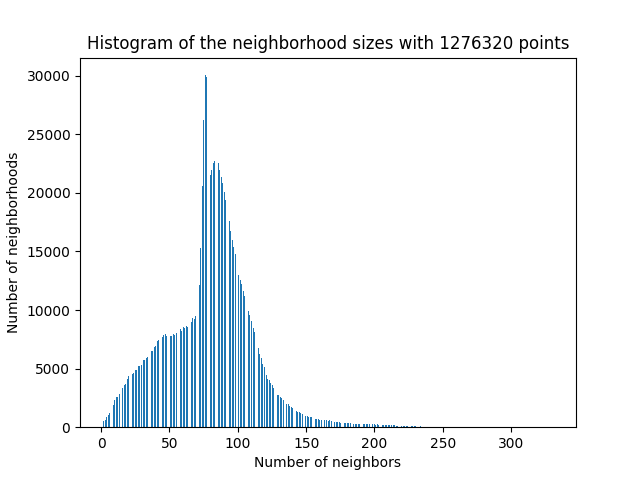
\includegraphics[width=\textwidth]{neigh_hist_scale0.png}
        \caption{$s=0$, $r=0.5m$}
    \end{subfigure}
    \hfill
    \begin{subfigure}{0.5\textwidth}
        \centering
        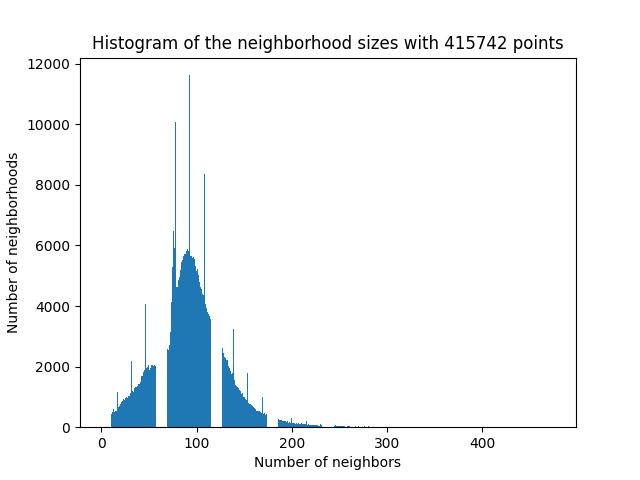
\includegraphics[width=\textwidth]{neigh_hist_scale1.png}
        \caption{$s=1$, $r=1m$}
    \end{subfigure}
    \hfill
    \begin{subfigure}{0.5\textwidth}
        \centering
        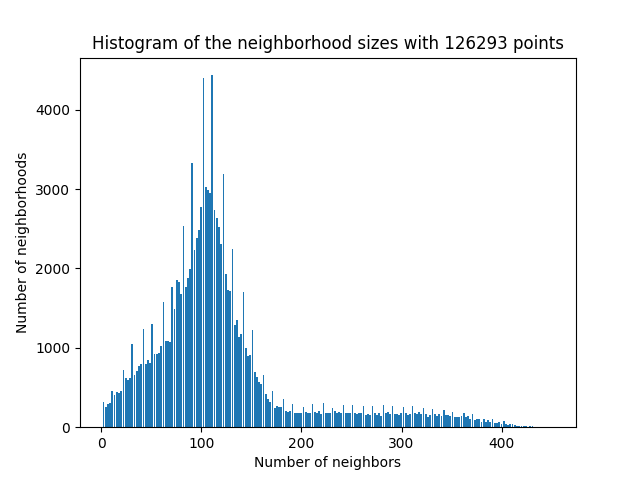
\includegraphics[width=\textwidth]{neigh_hist_scale2.png}
        \caption{$s=2$, $r=2m$}
    \end{subfigure}
    \hfill
    \begin{subfigure}{0.5\textwidth}
        \centering
        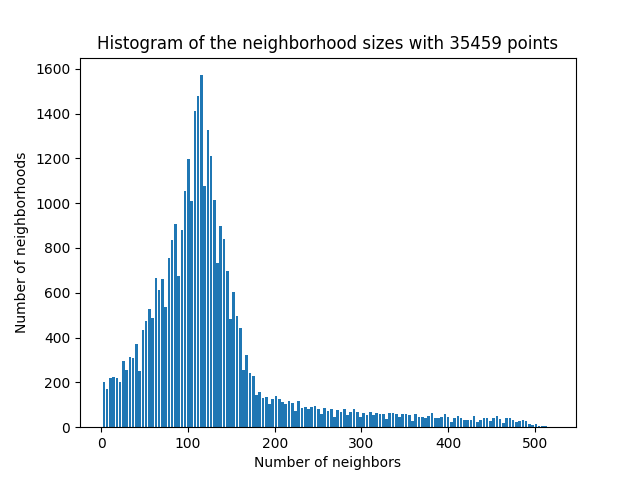
\includegraphics[width=\textwidth]{neigh_hist_scale3.png}
        \caption{$s=3$, $r=4m$}
    \end{subfigure}
    \caption{Histogram of the number of points in the neighborhood of each point for different scales $s$ on the subsampled Paris-rue-Cassette Dataset.}
    \label{fig:neigh_hist}
\end{figure}

\begin{table}
    \hspace*{-3.5cm}
    \begin{tabular}{cllllllll}
            Method & Ground & Building & Traffic Signs & Pedestrians & Cars & Vegetation & Motorcycles & Weighted IoU \\
            \hline
            \cite{thomas_semantic_2018} & $81.48 \pm 2.95$ & $0.71 \pm 0.08$ & $0.90 \pm 0.11$ & $0.93 \pm 0.02$ & $0.47 \pm 0.13$ & $0.82 \pm 0.05$ & $0.97 \pm 0.02$ & $0.79 \pm 0.04$ \\
            W height features & $83.16 \pm 2.23$ & $0.72 \pm 0.04$ & $0.97 \pm 0.05$ & $0.94 \pm 0.01$ & $0.50 \pm 0.13$ & $0.81 \pm 0.06$ & $0.95 \pm 0.03$ & $0.79 \pm 0.03$ \\
            W/O multi-scaling & $68.76 \pm 5.77$ & $0.43 \pm 0.03$ & $0.09 \pm 0.03$ & $0.71 \pm 0.02$ & $0.30 \pm 0.04$ & $0.63 \pm 0.03$ & $0.55 \pm 0.03$ & $0.55 \pm 0.02$ \\
            Knn neighborhood  & $71.87 \pm 8.28$ & $0.57 \pm 0.06$ & $0.48 \pm 0.27$ & $0.91 \pm 0.02$ & $0.37 \pm 0.08$ & $0.81 \pm 0.02$ & $0.87 \pm 0.02$ & $0.71 \pm 0.03$ \\
    \end{tabular}

    \caption{Benchmark results with Random Forest classifier}
    \label{tab:benchmark_RF}
\end{table}
\begin{table}
    \hspace*{-3.5cm}
    \begin{tabular}{cllllllll}
            Method & Ground & Building & Traffic Signs & Pedestrians & Cars & Vegetation & Motorcycles & Weighted IoU \\
            \hline
            \cite{thomas_semantic_2018} & $83.34 \pm 2.82$ & $0.70 \pm 0.06$ & $0.59 \pm 0.25$ & $0.93 \pm 0.02$ & $0.61 \pm 0.10$ & $0.78 \pm 0.06$ & $0.96 \pm 0.03$ & $0.80 \pm 0.03$ \\
            W height features & $84.94 \pm 2.38$ & $0.74 \pm 0.07$ & $0.82 \pm 0.18$ & $0.94 \pm 0.02$ & $0.59 \pm 0.12$ & $0.79 \pm 0.06$ & $0.98 \pm 0.01$ & $0.82 \pm 0.04$ \\
            W/O multi-scaling & $62.13 \pm 8.48$ & $0.41 \pm 0.04$ & $0.09 \pm 0.01$ & $0.71 \pm 0.03$ & $0.29 \pm 0.04$ & $0.67 \pm 0.02$ & $0.60 \pm 0.03$ & $0.55 \pm 0.02$ \\
            Knn neighborhood & $71.06 \pm 9.34$ & $0.56 \pm 0.09$ & $0.37 \pm 0.26$ & $0.94 \pm 0.02$ & $0.50 \pm 0.14$ & $0.81 \pm 0.04$ & $0.91 \pm 0.03$ & $0.74 \pm 0.03$ \\
    \end{tabular}
    \caption{Benchmark results with HBG classifier}
    \label{tab:benchmark_Boosting}
\end{table}

\subsection{Influence of neighborhood definition}
With spherical neighborhoods instead of KNN, the features always describe a part of the space of the same size at each scale.

\subsection{Influence of scales}

\subsection{Additional features and feature importance comparision}

Feature importances are computed as the mean and standard deviation of accumulation of the impurity decrease within each tree.  Impurity decrease is the reduction of the criterion value (such as entropy or gini index) when a feature is used to split a node in a decision tree. The importance of a feature is computed as the (normalized) total reduction of the criterion brought by that feature.

\begin{figure}
    \hspace*{-2cm}  
        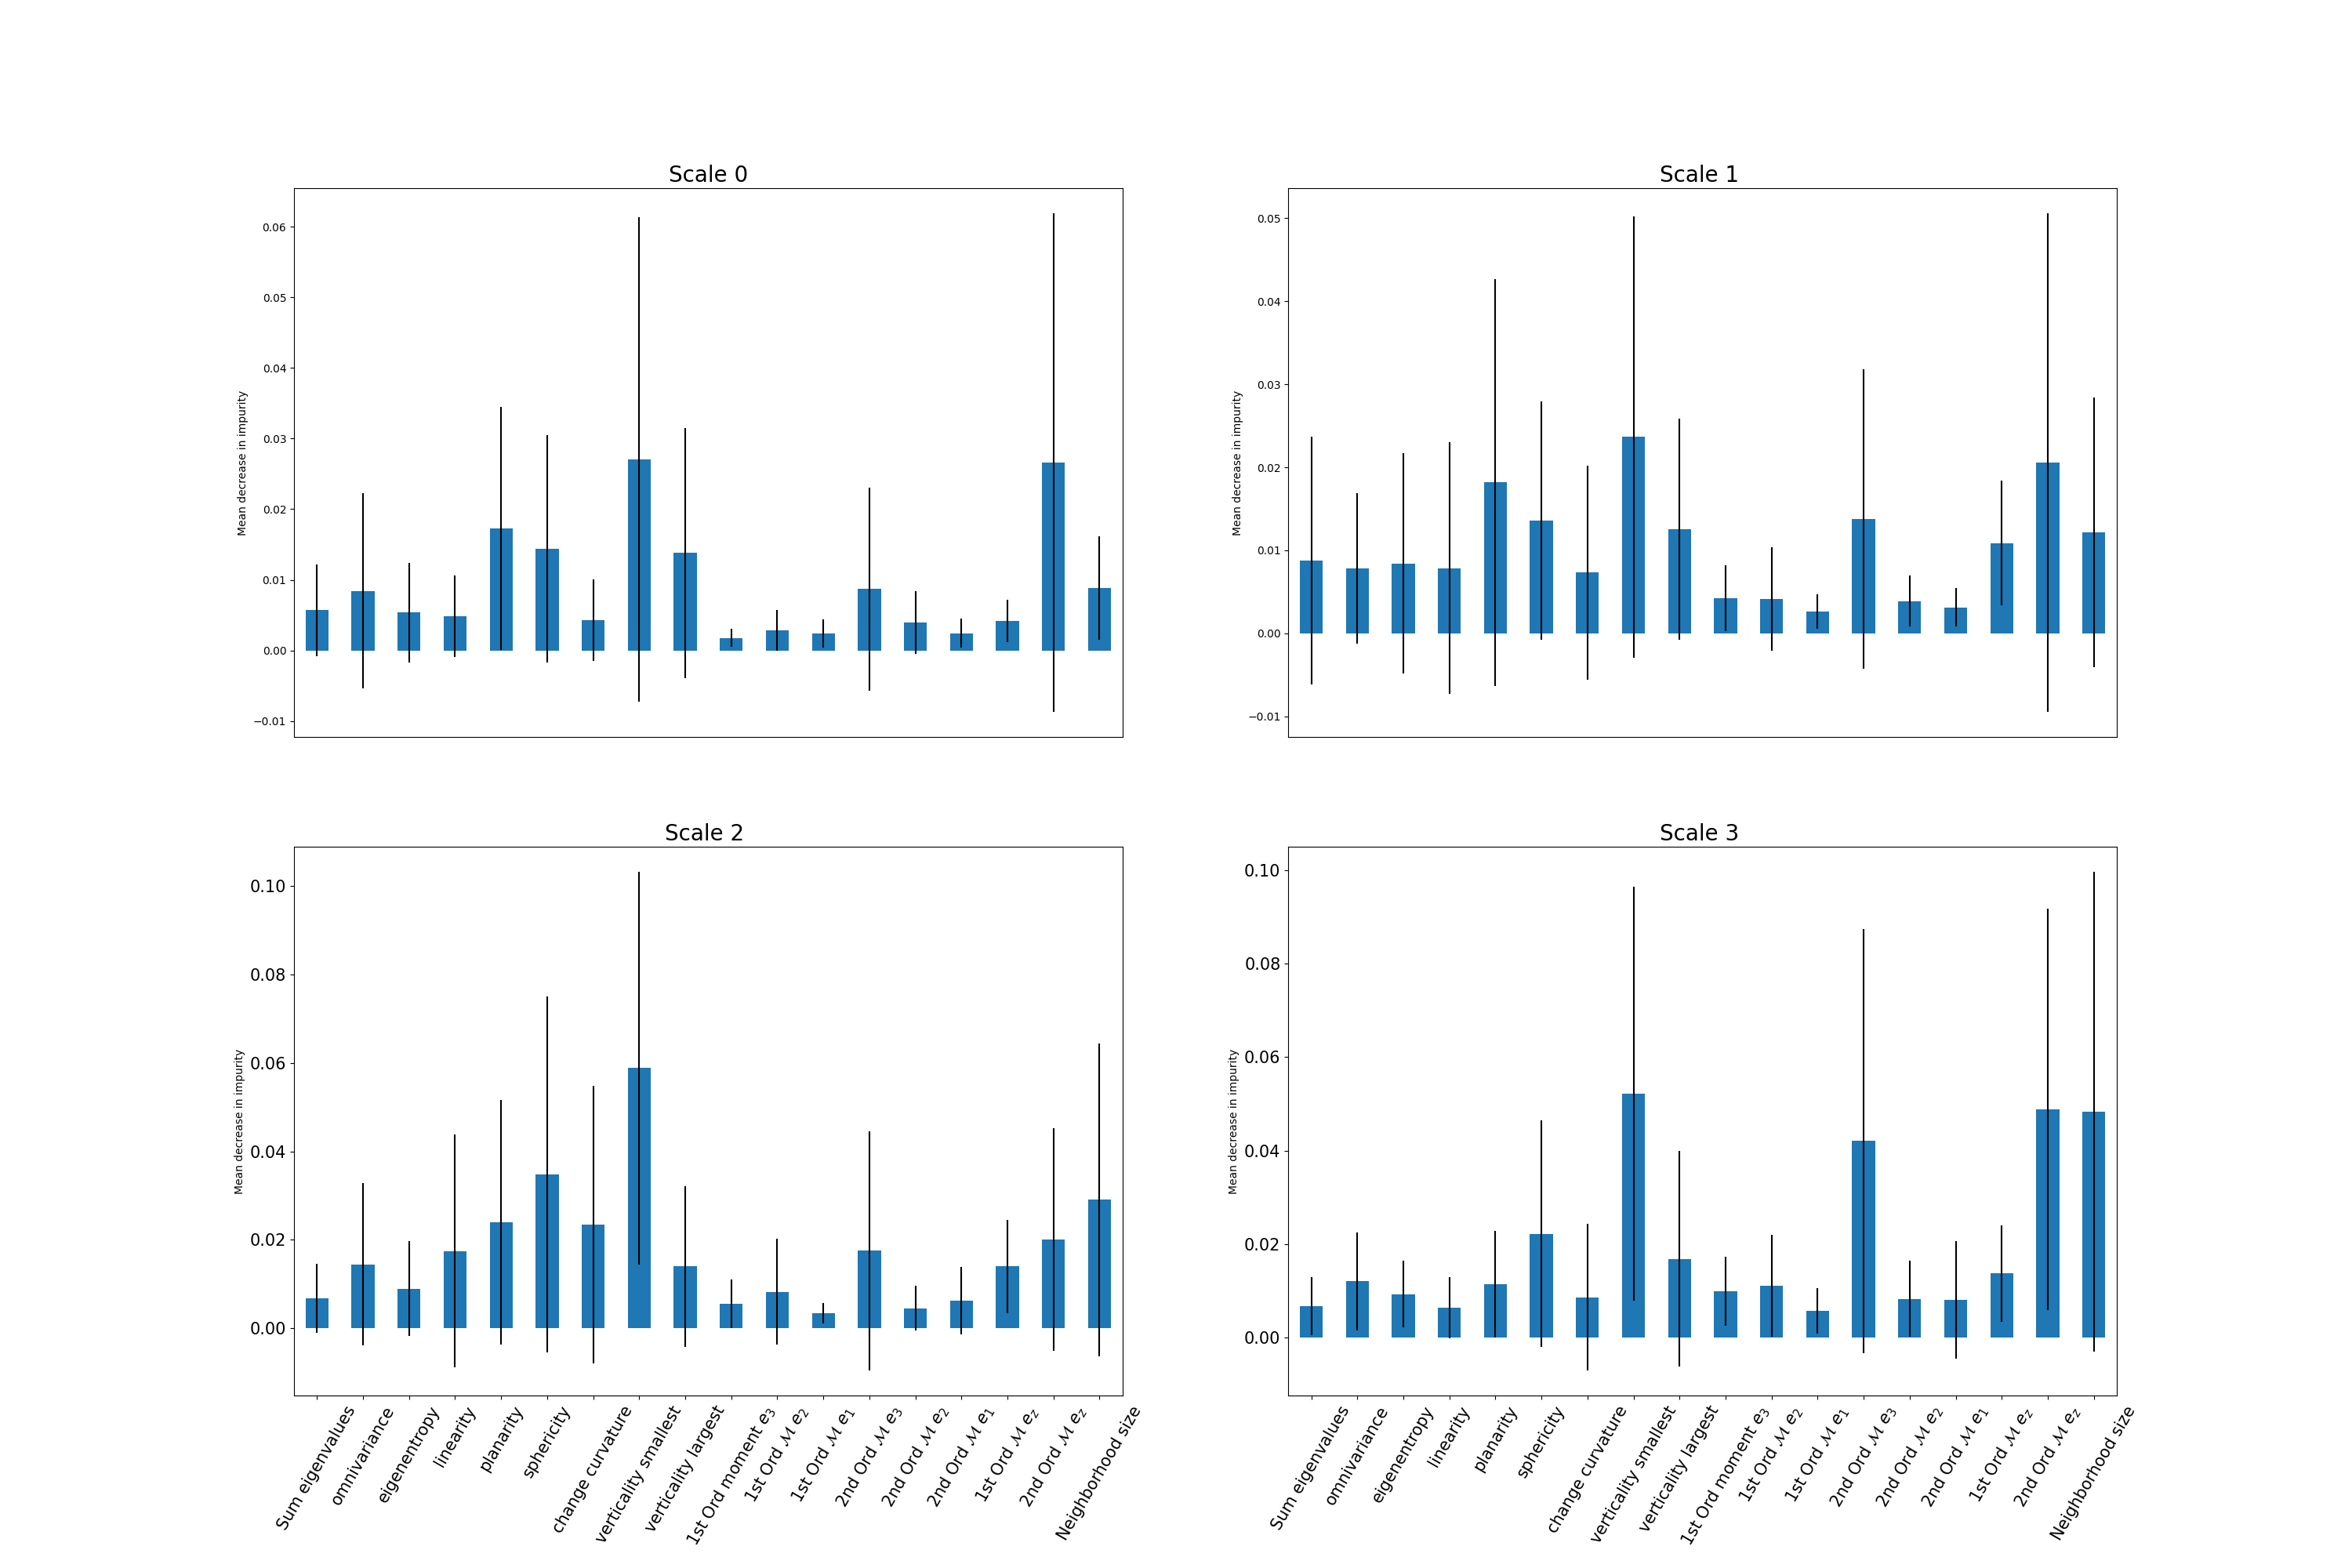
\includegraphics[width=1.3\textwidth]{MDI_feature_importances_DEFAULT.png}
        \caption{Mean decrease impurity feature importances with the 18 default features}
        \label{fig:MDI_default}
\end{figure}
\begin{figure}
    \hspace*{-2cm}
        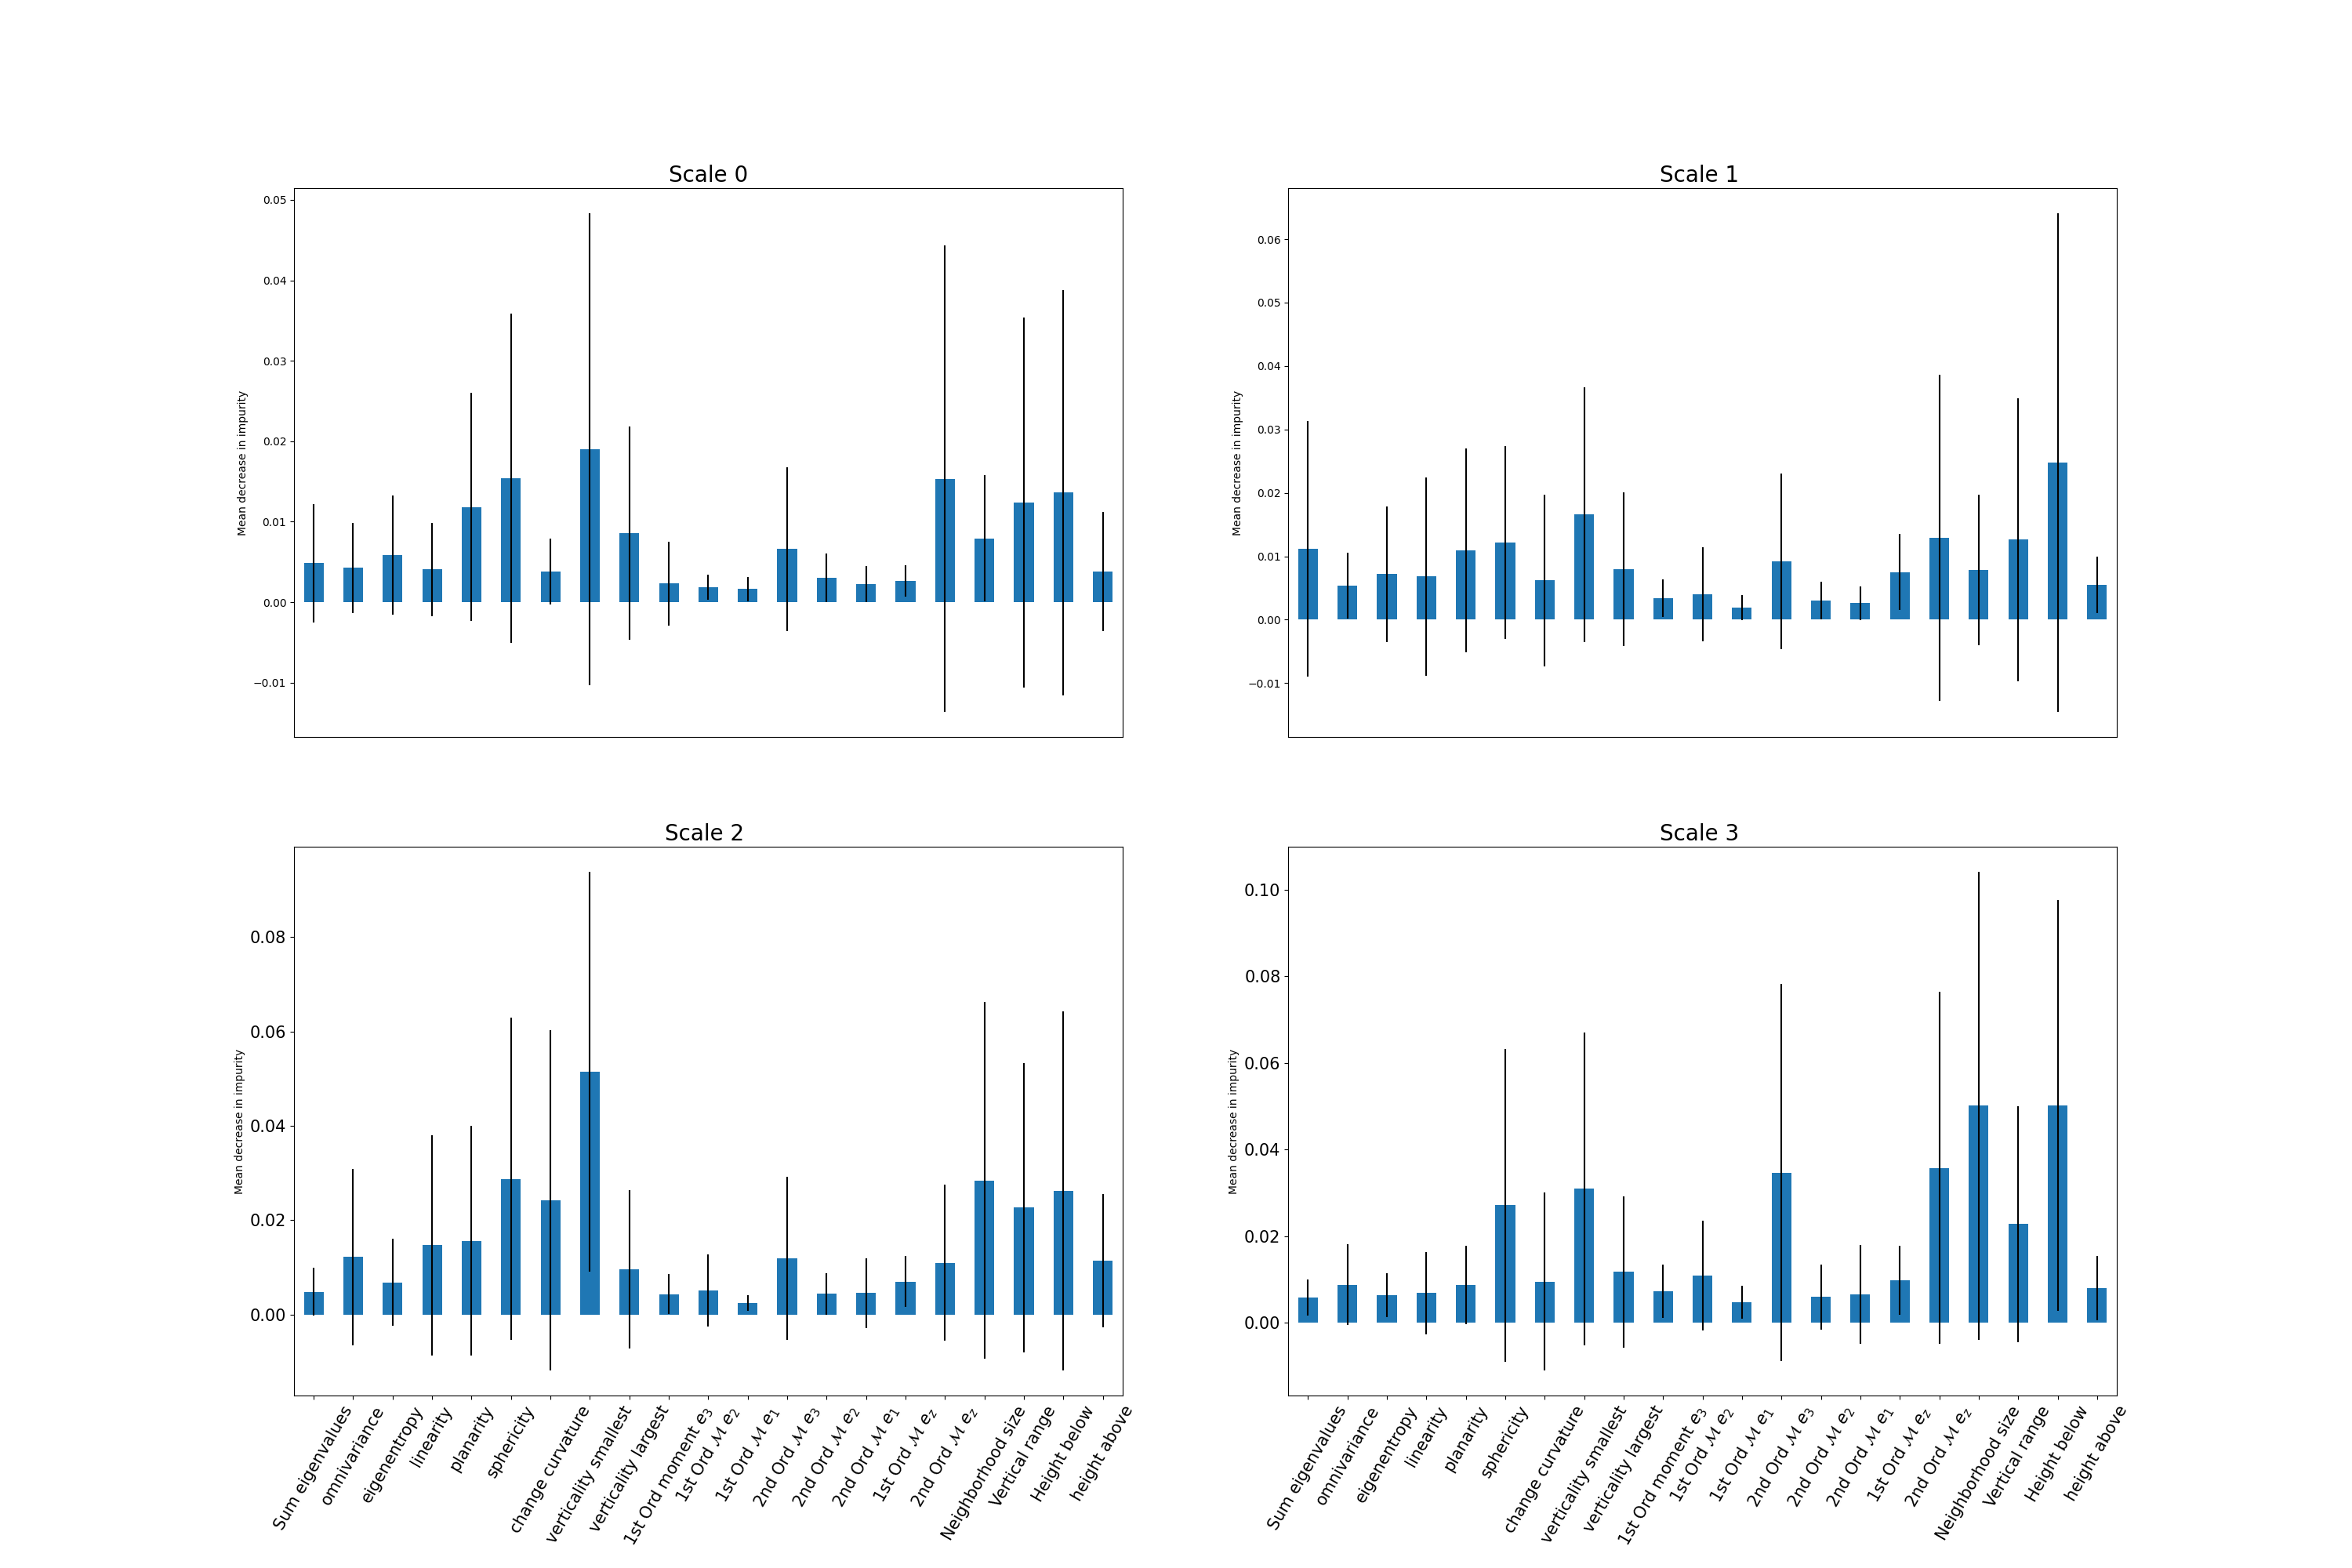
\includegraphics[width=1.3\textwidth]{MDI_feature_importances_W_HEIGHT_FEAT.png}
    \caption{Mean decrease impurity feature importances for the Paris-rue-Cassette dataset with additional height features (21 features in total).}
    \label{fig:MDI_height}
\end{figure}


Permutation feature importance is a model agnostic feature importance mehtod and is a commonly used technique to assess how much a feature is important to a classifier prediction. The idea is to assess how much the model's performance changes when modifying the value of the given feature. It is done by shuffling the values of the variable and observe the difference of the prediction accuracy.
Unlike the previous method, this approach is not biased by high-cardinality features.

\begin{figure}
    \hspace*{-2cm}
    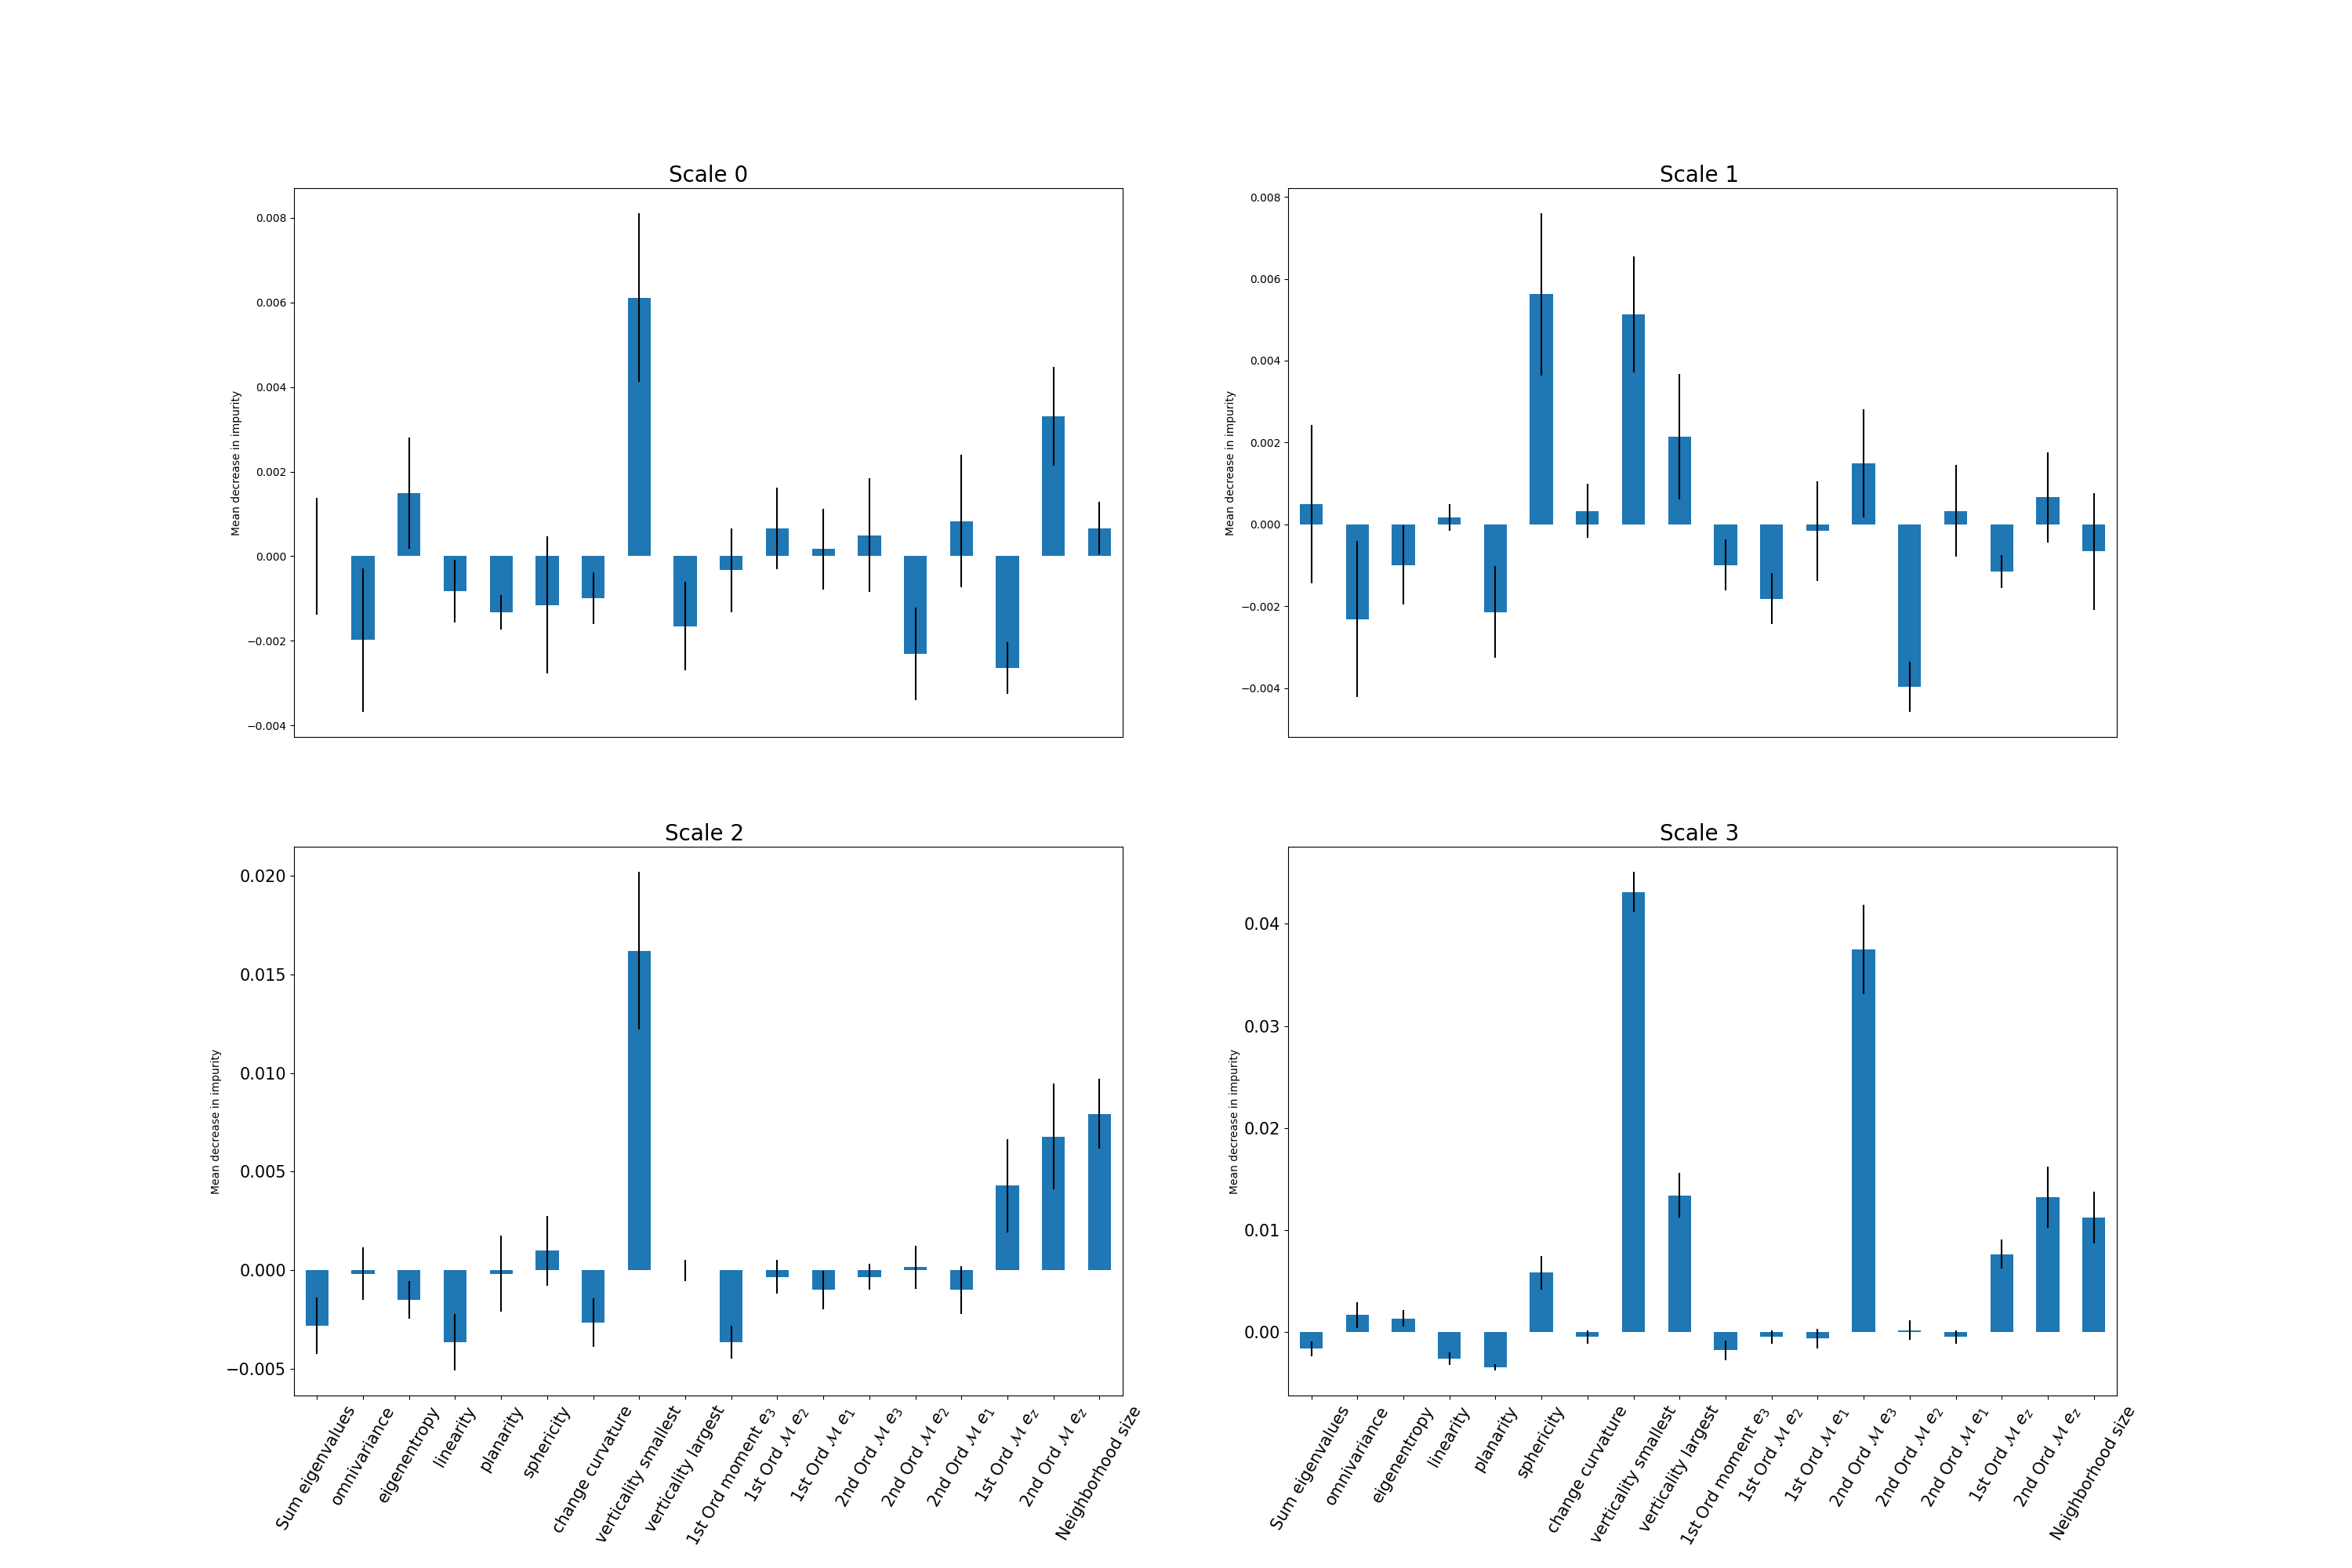
\includegraphics[width=1.3\textwidth]{permutation_feature_importances_DEFAULT.png}
    \caption{Permutation feature importances with th default 18 features}
    \label{fig:permutation_default}
\end{figure}
\begin{figure}
    \hspace*{-2cm}
        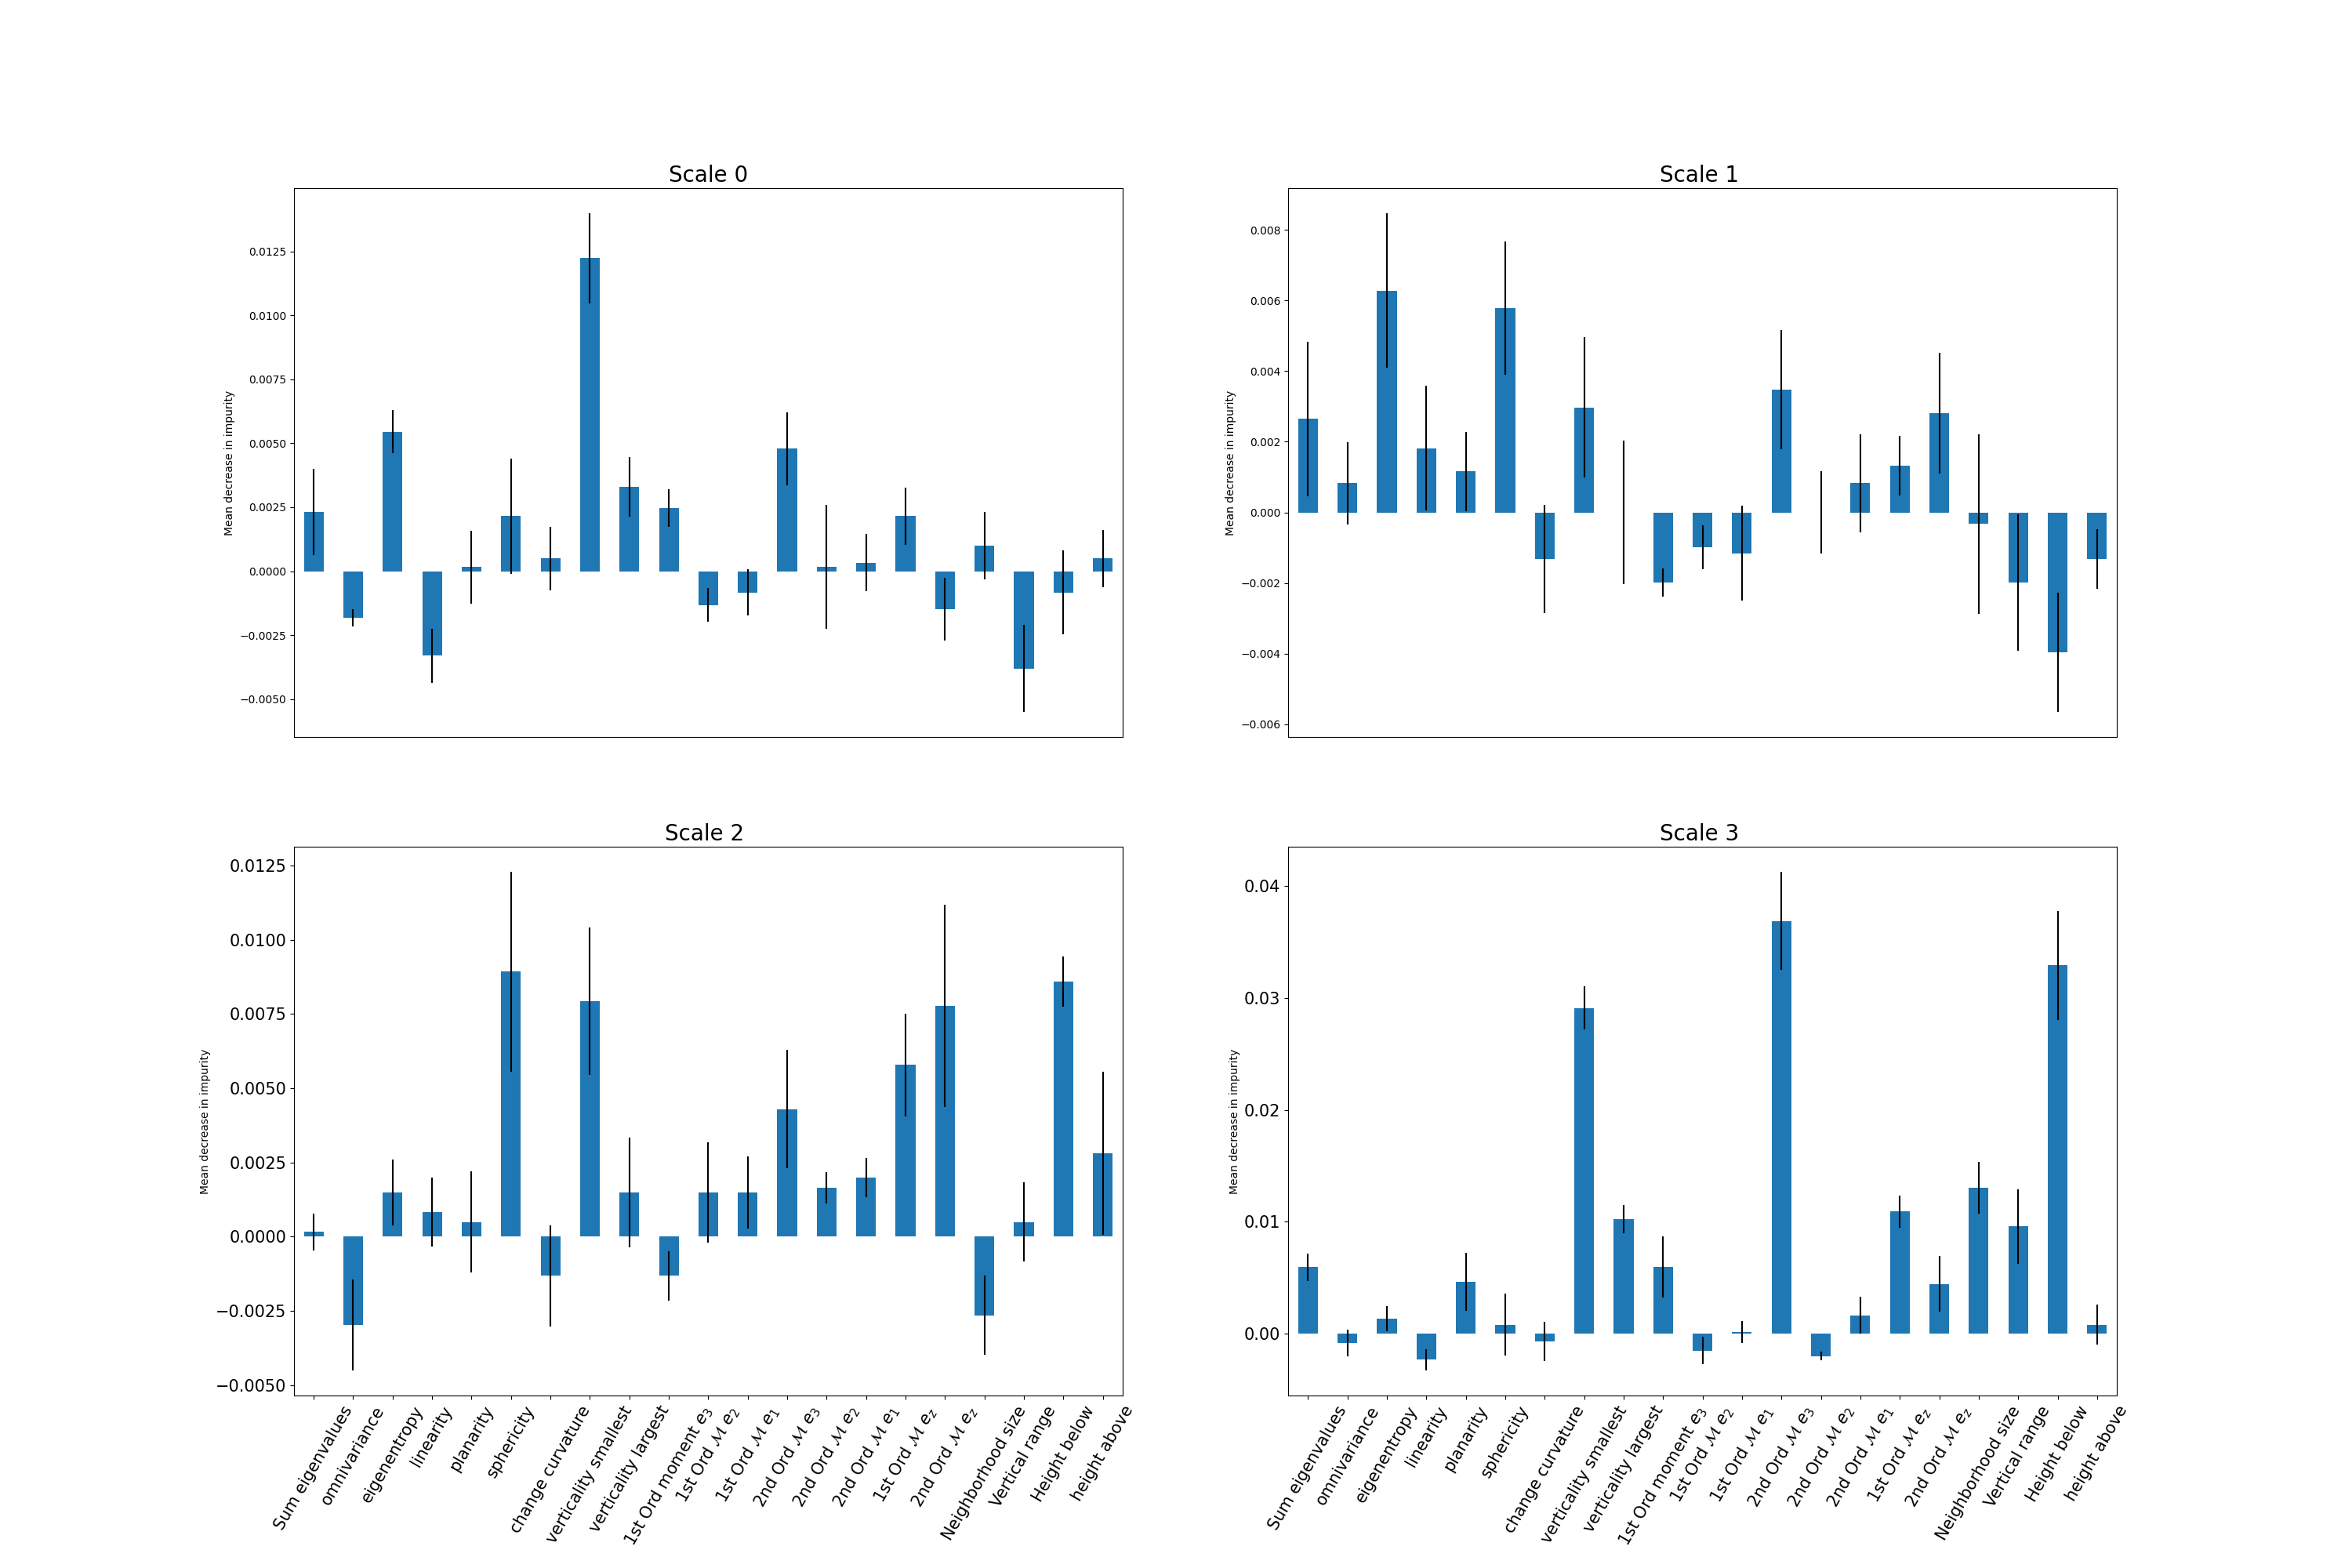
\includegraphics[width=1.3\textwidth]{permutation_feature_importances_W_HEIGHT_FEAT.png}
    \caption{Permutation feature importances for the Paris-rue-Cassette dataset with addition height features (21 features in total).}
    \label{fig:permutation_height}
\end{figure}

With a uniform density, the number of points in the neighborhood becomes a feature itself, describing the neighborhood occupancy rate. In Figure \ref{fig:MDI_default}, the number of points in the neighborhood is one the most important features, especially at the smallest scale. 

\subsection{NPM3D dataset}


\section{Improvement proposals}
\subsection{Speed up attempts}
I tried to compute the features on multiple CPU processes using \texttt{multiprocessing} package to speed for loops. Howerver, objects placed on multiprocessing queues are pickled, transferred over the queue, and then unpickled. The pickling and unpickling steps add overhead, and for large objects this overhead can be significant. This is because large objects require more data to be pickled and transferred, and the unpickling step requires reconstructing the entire object. 

Then, I tried Numba which is a just-in-time compiler for Python that works best on code that uses NumPy arrays and functions. Computing the features of 40 points with 4 scales on the subsampled points (about 1,288,215 points) took 54 seconds. I computed and saved the features of all points, excluding the points with label 0. It took in [time ] hours. 

\subsection{Active learning}

\subsection{Classification methods}\label{sec:classification}
Random Forest classifier is usually used for semantic classification of 3D point clouds \cite{thomas_semantic_2018,hackel_fast_nodate}. Indeed, it is directly applicable to multi-class problems and has been shown to yield good results in reasonable time on large point clouds \cite{weinmann_semantic_2015,atik_machine_2021}. I use Gini index as splitting criterion.

However, other classification methods could be considered \cite{atik_machine_2021}. 

Boosting is an ensemble machine learning approach. Boosting algorithms combine multiple low accuracy or weak models to create high accuracy or strong model. Among the most popular boosting algorithms are AdaBoost, Gradient Boosting, and XGBoost.

\section{Conclusion}

In 2019, Thomas et al. \cite{thomas_kpconv_2019} propose a deep learning approach for semantic segmentation using convolutions on point clouds.

\medskip
\bibliographystyle{plain}
\bibliography{ref}

\appendix

\section{Multiscale features computation}


\end{document}